\documentclass[11pt, aspectratio = 169]{beamer}

% \usepackage{sgamevar}
% \renewcommand{\gamestretch}{2.5}

\definecolor{good_red}{RGB}{136, 0, 17}
\definecolor{good_blue}{RGB}{0, 100, 125}

\definecolor{color1}{RGB}{0, 143, 248}
\definecolor{color2}{RGB}{151, 165, 52}
\definecolor{color3}{RGB}{231, 105, 20}
\definecolor{color4}{RGB}{205, 182, 50}
\definecolor{color5}{RGB}{25, 102, 137}
\definecolor{color6}{RGB}{211, 186, 112}
\definecolor{color7}{RGB}{226, 126, 88}

%\usetheme{CoeCollege1}
\usetheme{CoeCollege2}
%\usetheme{softTeal}

\pgfplotsset{compat=1.18}

\title[Carbon Pricing \& Environmental Inequality]{The Implications of Carbon Pricing\\ for Environmental Inequality}
% \subtitle{Senior Thesis Defense}
\author{Evan Perry}
\date{\today}

\begin{document}

\maketitlepage

\begin{frame}{Preliminaries}
    
\begin{itemize}
    \item Thank yous and apologies
    \vfill
    \item Revisions (based on feedback) since 2023-04-20:
    \begin{itemize}
        \item Copyediting
        \item Acknowledgements
        \item 5.3 \quad Results --- expanded discussion of EI Gap
        \item 5.4 \quad Diagnostics \& Limitations
    \end{itemize}
    \vfill
    \item Slides \& replication project available
\end{itemize}


\end{frame}


\begin{frame}{Overview}

\begin{block}{Research Question}
    Do carbon pricing policies exacerbate inequalities in air pollution concentrations?
\end{block}
\vfill

\begin{description}
    \item[Background] Carbon pricing policies are big globally, more common domestically, and popular amongst economists---but little is known about \emph{how} these policies affect the distribution of local air pollution
    \vfill
    \item[Method]  Study the effect of a carbon price on electricity generation in California on air pollution disparities across the Western US
    \begin{enumerate}
        \item Model: Build a model of carbon pricing and environmental inequality
        \item Simulation: Use the model and data to estimate environmental inequalities under a range of carbon prices
    \end{enumerate}
\end{description}
    
\end{frame}


\begin{frame}{Overview (contd.)}
    
\begin{description}
    \item[Results]\begin{itemize}
        \item Concentration of nitrous oxide emissions increases by  in disadvantaged communities, but decreases by in non-disadvantaged communities
        \item Sulfur dioxide \& particulate matter concentration disparities do not meaningfully change
        \item Effects are driven by differences in coverage under the regulation  
    \end{itemize}
    \vfill
    \item[Implications]\begin{itemize}
        \item Exposes potential flaw of ex-post analyses that look exclusively at the regulated geography
        \item Warrants additional research on combined cap-and-trade + localized pollution control policies
    \end{itemize}
\end{description}

\end{frame}


% \begin{frame}{Overview}
    
% \begin{block}{Research Question}
%     Do carbon pricing policies exacerbate inequalities in air pollution concentrations?
% \end{block}

% \vfill
% \begin{itemize}
%     \item Model: Predict investment, hourly generation, and hourly emissions outcomes for power plants, and use these to predict disparities in air pollution concentrations
%     \vfill 
%     \item Application: Simulate outcomes related to generation, emissions, and disparities in air pollution concentrations for the Western US
% \end{itemize}

% \end{frame}

\sectiontocslide{Introduction \& Motivation}

% \begin{frame}{Climate Change is Bad}
    
% \begin{quote}
%     It is unequivocal that human influence has warmed the atmosphere, ocean and land. Widespread and rapid changes in the atmosphere, ocean, cryosphere and biosphere have occurred. \citep{ipcc1_summary}
% \end{quote}

% \vfill
% \begin{itemize}
%     \item Greenhouse gas emissions---particularly CO$_2$---drive climate change 
%     \item Threatens ecosystems, infrastructure, living standards, public health, and peace
%     \item Climate damages per tonne of CO$_2$: \$185
%     \item 2021 US Emissions: 6.34 billion tonnes CO$_2$e
% \end{itemize}

% \end{frame}


% \begin{frame}{Background on Carbon Pricing}

% \begin{columns}
% \begin{column}{0.5\textwidth}
%     \centering 
%     The Market for Emissions
%     \footnotesize
%     \vfill
%     \begin{tikzpicture}[scale=0.4]
%         \draw[very thick, <->] (0,10) node[left]{$p$} -- (0,0) -- (13,0);	
%         \draw[very thick, color2, domain=0:12] plot(\x, {7.6 - .6*\x}) node[above right]{\footnotesize D = MB};
%         \draw[very thick, color1, domain=0:12] plot(\x, {4.6 + .4*\x}) node[right]{\footnotesize S = MSC};
%         \draw[very thick] (11, 0) node[below]{$E_\text{Current}$} -- (11, 10);
%         \draw[very thick, lightgray] (3,0) node[below, black]{$E^*$} -- (3,10);
%         \draw[very thick, lightgray] (0,5.8) node[left, black]{$p^*$} -- (13,5.8);	
%         \node[below] at (6.5, -3) {CO$_2$e Emissions ($E$)};
%         \draw (7, -2) node{$\underbrace{~~~~~~~~~~~~~~~~~~~~~~~~~~~~~~~}_{A^*}$};
%     \end{tikzpicture}
% \end{column}
% \begin{column}{0.5\textwidth}
%     \centering
%     Cost-Minimizing Abatement
%     \footnotesize
%     \vspace*{1em}
%     \begin{tikzpicture}[scale=0.5]
%         \fill[lightgray!50!, domain = 0:7, variable = \x] (0,0) -- plot(\x, {.09*\x^2}) -- (7,0) -- cycle;
%         \fill[lightgray!50!, domain = 7:10, variable = \x] (7,0) -- plot(\x, {.1*(12-\x)^2 + 1.91}) -- (10,0) -- cycle;
%         \draw (0,0) rectangle (10,8.33);
%         \draw (0,0) node[below]{0} -- (10,0) node[below]{100} -- (10,8.33) node[above]{0} -- (0,8.33) node[above]{100} -- (0,0);
%         \draw[very thick, ->] (10, 9.33) -- (0, 9.33) node[pos=.5, above]{Polluter 2's Abatement (tonnes)};
%         \draw[very thick, ->] (0, -1) -- (10, -1) node[pos=.5, below]{Polluter 1's Abatement (tonnes)};
%         \draw[very thick, color2, domain=0:9.603] plot(\x, {.09*\x^2});
%         \draw[very thick, color1, domain=3.988:10] plot(\x, {.1*(12-\x)^2 + 1.91}); 
%         \draw[thick, dashed] (0,4.41) node[left]{\$50} -- (7,4.41);
%         \draw[thick, dashed] (7,8.33) node[above]{30} -- (7,0) node[below]{70};
%         \draw[thick, dashed] (5,8.33) node[above]{50} -- (5,0) node[below]{50};
%         \node[rotate=90, above] at (-1, 4.155) {Price (\$)};
%         \node[color2] at (9, 5.5) {MAC$_1$};
%         \node[color1] at (9, 1.5) {MAC$_2$};
%         % \draw[lightgray, thick] (5,0) node[below, black]{50} -- (5,8.33) node[above, black]{50};
%     \end{tikzpicture}
% \end{column}
% \end{columns}

% \end{frame}


\begin{frame}{Carbon Pricing}

\centering
Market for Emissions \\
\vspace*{1em}
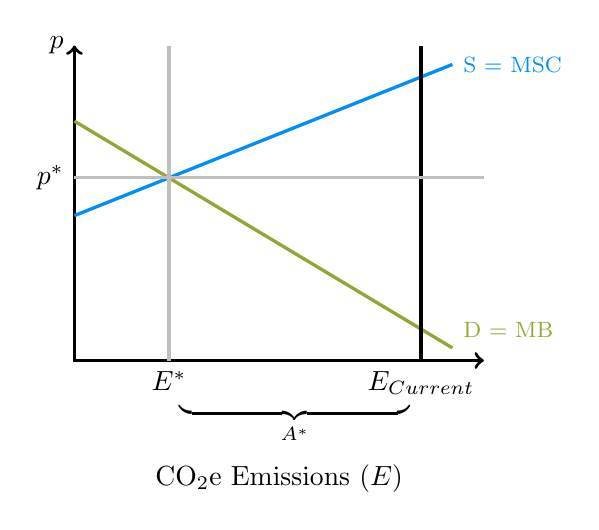
\begin{tikzpicture}[scale=0.4]
    \draw[very thick, <->] (0,10) node[left]{$p$} -- (0,0) -- (13,0);	
    \draw[very thick, color2, domain=0:12] plot(\x, {7.6 - .6*\x}) node[above right]{\footnotesize D = MB};
    \draw[very thick, color1, domain=0:12] plot(\x, {4.6 + .4*\x}) node[right]{\footnotesize S = MSC};
    \draw[very thick] (11, 0) node[below]{$E_\text{Current}$} -- (11, 10);
    \draw[very thick, lightgray] (3,0) node[below, black]{$E^*$} -- (3,10);
    \draw[very thick, lightgray] (0,5.8) node[left, black]{$p^*$} -- (13,5.8);	
    \node[below] at (6.5, -3) {CO$_2$e Emissions ($E$)};
    \draw (7, -2) node{$\underbrace{~~~~~~~~~~~~~~~~~~~~~~~~~}_{A^*}$};
\end{tikzpicture}
    
\end{frame}


\begin{frame}{Emissions Leakage}
  
\footnotesize
\centering
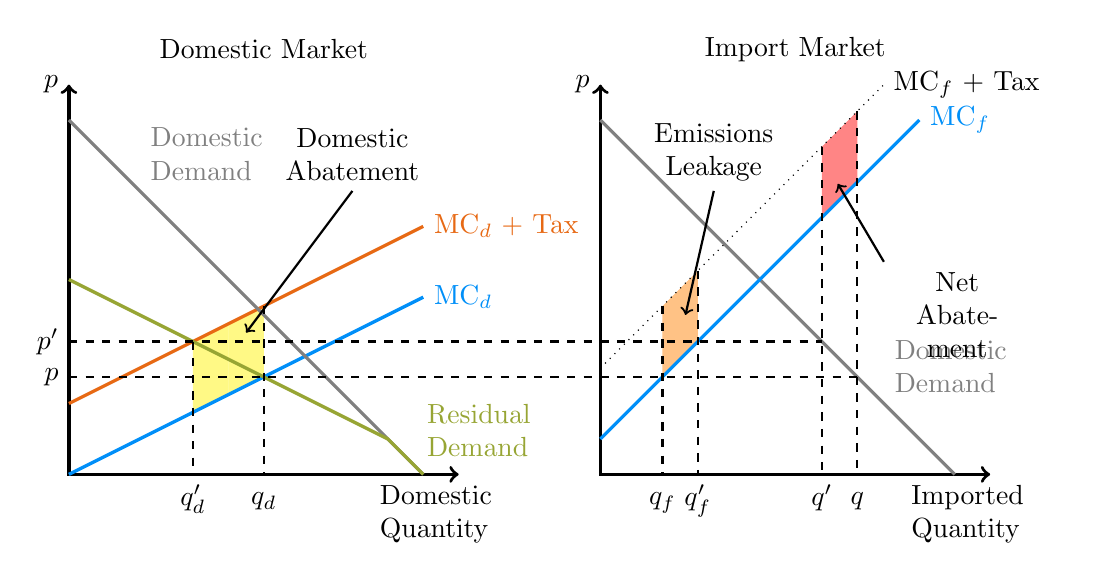
\begin{tikzpicture}[scale = 0.45]
    \draw[very thick, <->] (0, 11) node[left]{$p$} -- (0, 0) -- (11, 0) node[below, text width = 2cm]{Domestic Quantity};
    \draw[very thick, <->] (15, 11) node[left]{$p$} -- (15,0) -- (26, 0) node[below, text width = 2cm]{Imported Quantity};
    \fill[yellow!80!, opacity = 0.6] (3.5, 3.75) -- (3.5, 1.75) -- (4.5, 2.25) -- (4.5, 4.25) -- cycle;
    \fill[yellow!80!, opacity = 0.6] (4.5, 2.25) -- (5.5, 2.75) -- (5.5, 4.75) -- (4.5, 4.25) -- cycle;
    \fill[orange!80!, opacity = 0.6] (16.75, 4.75) -- (16.75, 2.75) -- (17.75, 3.75) -- (17.75, 5.75) -- cycle;
    %\fill[orange!80!, opacity = 0.6] (16.25, 4.25) -- (16.25, 2.25) -- (16.75, 2.75) -- (16.75, 4.75) -- cycle;
    \fill[red!80!, opacity = 0.6] (21.25, 9.25) -- (21.25, 7.25) -- (22.25, 8.25) -- (22.25, 10.25) -- cycle;
    %\fill[red!80!, opacity = 0.6] (20.75, 8.75) -- (20.75, 6.75) -- (21.25, 7.25) -- (21.25, 9.25) -- cycle;
    \draw[very thick, color1] (0,0) -- (10, 5) node[right]{MC$_d$};
    \draw[very thick, color3] (0,2) -- (10, 7) node[right]{MC$_d$ $+$ Tax};
    \draw[very thick, gray] (0, 10) -- (10,0) node[pos=.2, above right,text width = 1.5cm]{Domestic Demand}; 
    \draw[very thick, color2] (0,5.5) -- (9, 1) -- (10, 0) node[pos=.8, above right, text width = 1.5cm]{Residual Demand};
    %\draw[very thick, color2] (0, 6.5) -- (7,3) -- (10, 0);
    \draw[very thick, gray] (15, 10) -- (25, 0) node[pos=.8, above right,text width = 1.5cm]{Domestic Demand}; 
    \draw[very thick, color1] (15, 1) -- (24, 10) node[right, text width = 1.5cm]{MC$_f$};
    \draw[dashed, thick] (5.5, 4.75) -- (5.5, 0) node[below, yshift = -3pt]{$q_d$};
    \draw[dashed, thick] (3.5, 3.75) -- (3.5, 0) node[below]{$q_d'$};
    %\draw[dashed, thick] (4.5, 4.25) -- (4.5, 0) node[below]{$q_d''$};
    \draw[dashed, thick] (0, 3.75) node[left]{$p'$} -- (21.25, 3.75);
    \draw[dashed, thick] (0, 2.75) node[left]{$p$} -- (22.25, 2.75);
    %\draw[dashed, thick] (0,4.25) node[left]{$p''$} -- (20.75, 4.25);
    \draw[dashed, thick] (16.75,4.75) -- (16.75, 0) node[below, yshift = -3pt]{$q_f$};
    \draw[dashed, thick] (17.75, 5.75) -- (17.75, 0) node[below]{$q_f'$};
    %\draw[dashed, thick] (16.25, 4.25) -- (16.25, 0) node[below]{$q_f''$};
    \draw[dashed, thick] (22.25, 10.25) -- (22.25, 0) node[below, yshift = -3pt]{$q$};
    \draw[dashed, thick] (21.25, 9.25) -- (21.25, 0) node[below]{$q'$};
    %\draw[dashed, thick] (20.75, 8.75) -- (20.75, 0) node[below]{$q''$};
    \draw[dotted] (15, 3) -- (23, 11) node[right]{MC$_f$ $+$ Tax};
    \draw[thick, <-] (5, 4) -- (8, 8) node[above, text width = 2cm, align=center]{Domestic Abatement};
    \draw[thick, <-] (17.4, 4.5) -- (18.2, 8) node[above, text width = 2cm, align=center]{Emissions Leakage}; 
        \draw[thick, <-] (21.7, 8.2) -- (23, 6) node[below right, text width = 1.6cm, align=center]{Net Abatement};
        \node at (5.5, 12) {Domestic Market};
        \node at (20.5, 12) {Import Market}; 
\end{tikzpicture}

\end{frame}


\begin{frame}{Gobal Air Pollution v. Local Air Pollution}
    
    \begin{columns}
    \begin{column}{0.5\textwidth}
        \textbf{Global Air Pollutants}
        \vspace*{1em}
        \begin{itemize}
            \item Carbon dioxide (CO$_2$), Methane (CH$_4$), Nitrous oxide (N$_2$O)
            \vspace*{2em}
            \item Primarily long-run consequences
            \vspace*{2em}
            \item Location does not matter
        \end{itemize}
    \end{column}
    \begin{column}{0.5\textwidth}
        \textbf{Local Air Pollutants}
        \vspace*{1em}
        \begin{itemize}
            \item Nitrogen oxides (NO$_x$), Sulfur dioxide (SO$_2$), Particulate matter (PM2.5)
            \vspace*{1em}
            \item Mix of long- and short-run consequences
            \vspace*{1em}
            \item Location does matter
        \end{itemize}
    \end{column}
    \end{columns}
    
\end{frame}
    

\begin{frame}{Motivation \& Ex-Post Research}
    
    \begin{itemize}
        \item \href{https://ww2.arb.ca.gov/resources/documents/faq-cap-and-trade-program}{CARB Cap-and-Trade FAQ Page} 
        \vfill 
        \item Descriptive Analysis: Yes, California's cap-and-trade program increased disparities \citep{cushing2018carbon, pastor2022up}
        \vfill
        \item Causal Analysis: No, California's cap-and-trade program decreased disparities \citep{hernandez2023environmental}
    \end{itemize}

\end{frame}


\begin{frame}{Methodological Contributions}
    
\begin{itemize}
    \item Ex-ante model to anticipate changes in air pollution disparities
    \vfill 
    \item \emph{How} do carbon pricing policies shift local air pollution across jurisdictions?
    \vfill
    \item \cite{weber2021dynamic} creates a similar model, but does not:
    \begin{enumerate}
        \item Formally model disparities in air pollution concentrations
        \item Consider leakage and the redistribution outside of California
    \end{enumerate}
\end{itemize}

\end{frame}

% \begin{frame}{}
    
% \begin{itemize}
%     \item \emph{How} do carbon pricing policies lead to changes in air pollution concentration disparities?
%     \vfill 
%     \item \emph{How} do carbon pricing policies shift local air pollution across jurisdictions?
%     \vfill 
%     \item Contributions:
%     \begin{itemize}
%         \item Predictive framework for the effect of carbon pricing within the electric power industry on local air pollution disparities 
%         \item Demonstrate the importance of considering disparities across jurisdictions
%     \end{itemize}
% \end{itemize}

% \end{frame}


\sectiontocslide{Modeling Carbon Pricing \& Environmental Inequality}


\begin{frame}{Model Overview}

\begin{description}
    \item[Agents] $N$ fossil fuel power plants
    \vfill
    \item[Environ.]\begin{itemize}
        \item Geography: $R$ regions, each with its own wholesale market for electricity
        \item Constraints: Demand, (Capacity,) Transmission
        \item Markets: Perfectly competitive
    \end{itemize}  
    \vfill 
    \item[Actions]\begin{enumerate}
        \item Initial investment decision
        \item Hourly generation decisions
    \end{enumerate}
    \vfill
    \item[Behavior] Maximize discounted sum of future profits
    \vfill
    \item[Equilibrium] Minimize total investment and generation costs $\to$ Generation outcomes $\to$ Air pollution disparity outcomes 
\end{description}

\end{frame}


\begin{frame}{}
    
\end{frame}



\sectiontocslide{Empirical Strategy \& Data}


\begin{frame}{Empirical Strategy: Simulation}
    
\begin{columns}
    \begin{column}{0.5\textwidth}
    
    \begin{itemize}
        \item Simulate generation across the Western US power grid (Western Interconnection)
        \vspace*{1em}
        \item Focus only on fossil fuel generation: coal, (natural) gas, oil
    \end{itemize}    

    \end{column}
    \begin{column}{0.5\textwidth}
        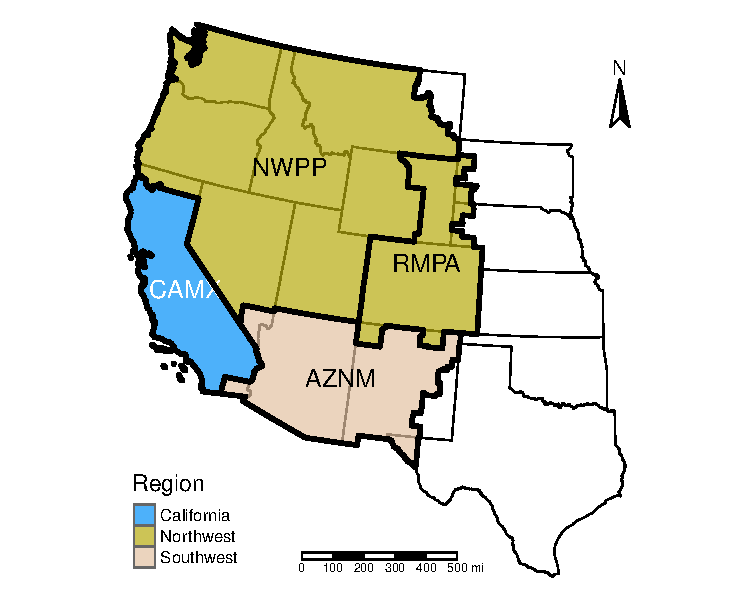
\includegraphics[width = \textwidth]{figures/chapter3_figures/WECC_map.pdf}
    \end{column}
\end{columns}

\end{frame}


\begin{frame}{Empirical Strategy: Policy Scenarios}
    
    \begin{columns}
        \begin{column}{0.5\textwidth}
            \begin{itemize}
                \item Border Carbon Adjustments (BCAs): ``Carbon tariff'' on electricity California imports from elsewhere
                \vspace*{1em}
                \item Nine policy scenarios with a combination of BCAs and carbon prices
            \end{itemize}
        \end{column}
        \begin{column}{0.5\textwidth}
            \footnotesize
            \centering
            \begin{tabular}{c c c}
                \hline\hline
                Scenario & BCA? & Tax (\$/tonne)\\
                \hline
                A & No & 0\\
                B & No & 20\\
                C & No & 40\\
                D & No & 60\\
                E & No & 80\\
                F & Yes & 20 \\
                G & Yes & 40 \\
                H & Yes & 60 \\
                I & Yes & 80 \\
            \hline    
            \end{tabular}
        \end{column}
    \end{columns}

\end{frame}


\begin{frame}{Empirical Strategy: $k$-Means Clustering}
    
\begin{itemize}
    \item Problem: Constrained optimization problems are too large
    \vfill
    \item Generation Problem
    \begin{itemize}
        \item Simplify $N$: $k$-means cluster power plants into thirty groups
    \end{itemize}
    \vfill 
    \item Investment Problem
    \begin{itemize}
        \item Simplify $T$: $k$-means cluster electricity demand into a ``representative day''
        \item Simplify $N$: $k$-means cluster generation clusters into four clusters
    \end{itemize}
\end{itemize}

\end{frame}


\begin{frame}{Empirical Strategy: Generation $\to$ Pollutant Concentrations}
    
\end{frame}



\begin{frame}{Data: Power Plant}
    
    \begin{itemize}
        \item 2019 Emissions \& Generation Resource Integrated Database (eGRID) from the EPA
        \item 
    \end{itemize}

\end{frame}


\begin{frame}{Data: Electricity Demand}
    
\end{frame}


\begin{frame}{Data: Disadvantaged Communities}
    
\end{frame}



\sectiontocslide{Simulation Results}


\begin{frame}{Generation}
    
\end{frame}


\begin{frame}{Greenhouse Gas Emissions}
    
\end{frame}


\begin{frame}{Local Air Pollutant Emissions}
    
\end{frame}


\begin{frame}{The EI Gap}

    \centering
    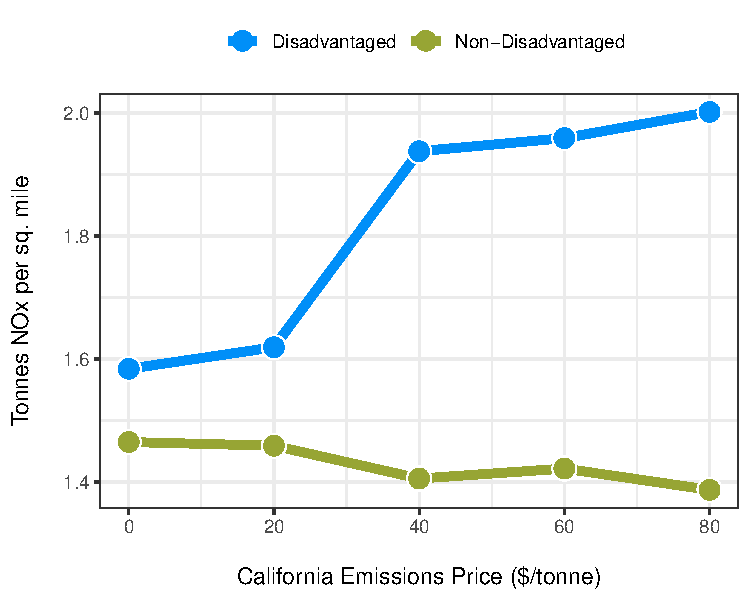
\includegraphics[width = 0.7\textwidth]{figures/chapter5_figures/ei_gap_bca_nox.pdf}

\end{frame}



\sectiontocslide{Takeaways \& Discussion}





\begin{frame}[allowframebreaks]{References}
\footnotesize

\bibliography{references}

\end{frame}



\end{document}